\chapter{Introduction}

This report describes the design and implementation of a hardware accelerator that performs the Sobel operator on an 8-bit monochrome image. Figure \ref{fig:SysArch} shows an overview of the system architecture. The input image is stored in external RAM and the output image is written back to the external RAM, but at a different memory location. Using the to two signals 'start' and 'finish', a four phase handshake protokol is used to start and finish the processing sequence.

\begin{figure}[H]
	\centering
	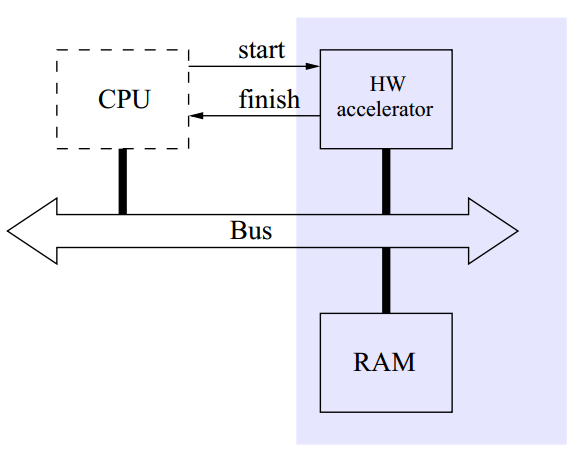
\includegraphics[width=0.5 \textwidth]{SystemArchitecture.png}
	\caption{System architecture as given by the lab assignment.}
	\label{fig:SysArch}
\end{figure}

